\documentclass[oneside, 11pt, ngerman, a4paper, biblography=totoc]{scrartcl}

%listof=totocnumbered,bibliography=totocnumbered,
% if using scrartcl: \setkomafont{sectioning}{\rmfamily\bfseries}

%%%%%%%%%%%%%%%%%%%%%%%%%%%%%%%%%%%%%%%%%%%%%%%%%%%%%%
% Usepackages						                 %
%%%%%%%%%%%%%%%%%%%%%%%%%%%%%%%%%%%%%%%%%%%%%%%%%%%%%%
\usepackage{packages} % Ruft die Datei packages.sty auf in der die eigentlichen usepackages geladen werden
%% If needed, add addiional Packages here

%%%%%%%%%%%%%%%%%%%%%%%%%%
% Modify Experiment Name %
%%%%%%%%%%%%%%%%%%%%%%%%%%

\newcommand{\VersuchsNummer}{Versuch X}
\newcommand{\VersuchsName}{Name des Versuchs}

\title{	\large Physikalisches Institut Universität Freiburg\\ % Your institution
	\large Hermann-Herder-Str. 3, 79104 Freiburg\\[5mm]
	\Large Anfänger Praktikum I \\[15mm] \Huge\textbf{\VersuchsNummer :\\ \VersuchsName}\\[15mm]}

%%%%%%%%%%%%%%%%%%%%%
% Modify Tutor Name %
%%%%%%%%%%%%%%%%%%%%%
\author{
	\large % Your Name
	From \textsc{Person1}\thanks{{\href{mailto:Person1@example.com}{Person1@example.com}}} ~und \textsc{Person2}\thanks{{\href{mailto:Person2@uni-freiburg.de}{Person2@uni-freiburg.de}}} \\
	\large (Gruppe XXX) \\[3mm]
	\large Assistant: \\[3mm] % Tutor name
	\large Datum: \\[3mm] % Tutor name
	%\vspace{-5mm}
}
\date{}

\begin{document}
	% Titlepage
	\maketitle
	\thispagestyle{empty}
	% Empty backside of Titlepage
	\newpage
	\thispagestyle{empty}
	\null
	\newpage

	% Table of Contents page
	\newpage
	\tableofcontents
	\newpage
	\thispagestyle{empty}
	\null
	\newpage

	%%%%%%%%%%%%%%%%%%%%%
	% Add Contents Here %
	%%%%%%%%%%%%%%%%%%%%%

	% im Ordner sections sind die Dateien für die Einzelnen Versuchsteile, die hier eingebunden werden.
	\section{Ziel des Versuchs}

	\section{Versuchsdurchführung}

	\section{Auswertung und Fehleranalyse}
	\section{Zusammenfassung und Diskussion}
	\newpage
	\section{Anhang}
\subsection{Zusätzliche Plots}
	\newpage
	\section{Laborheft}
\begin{figure}[H]
    \centering
    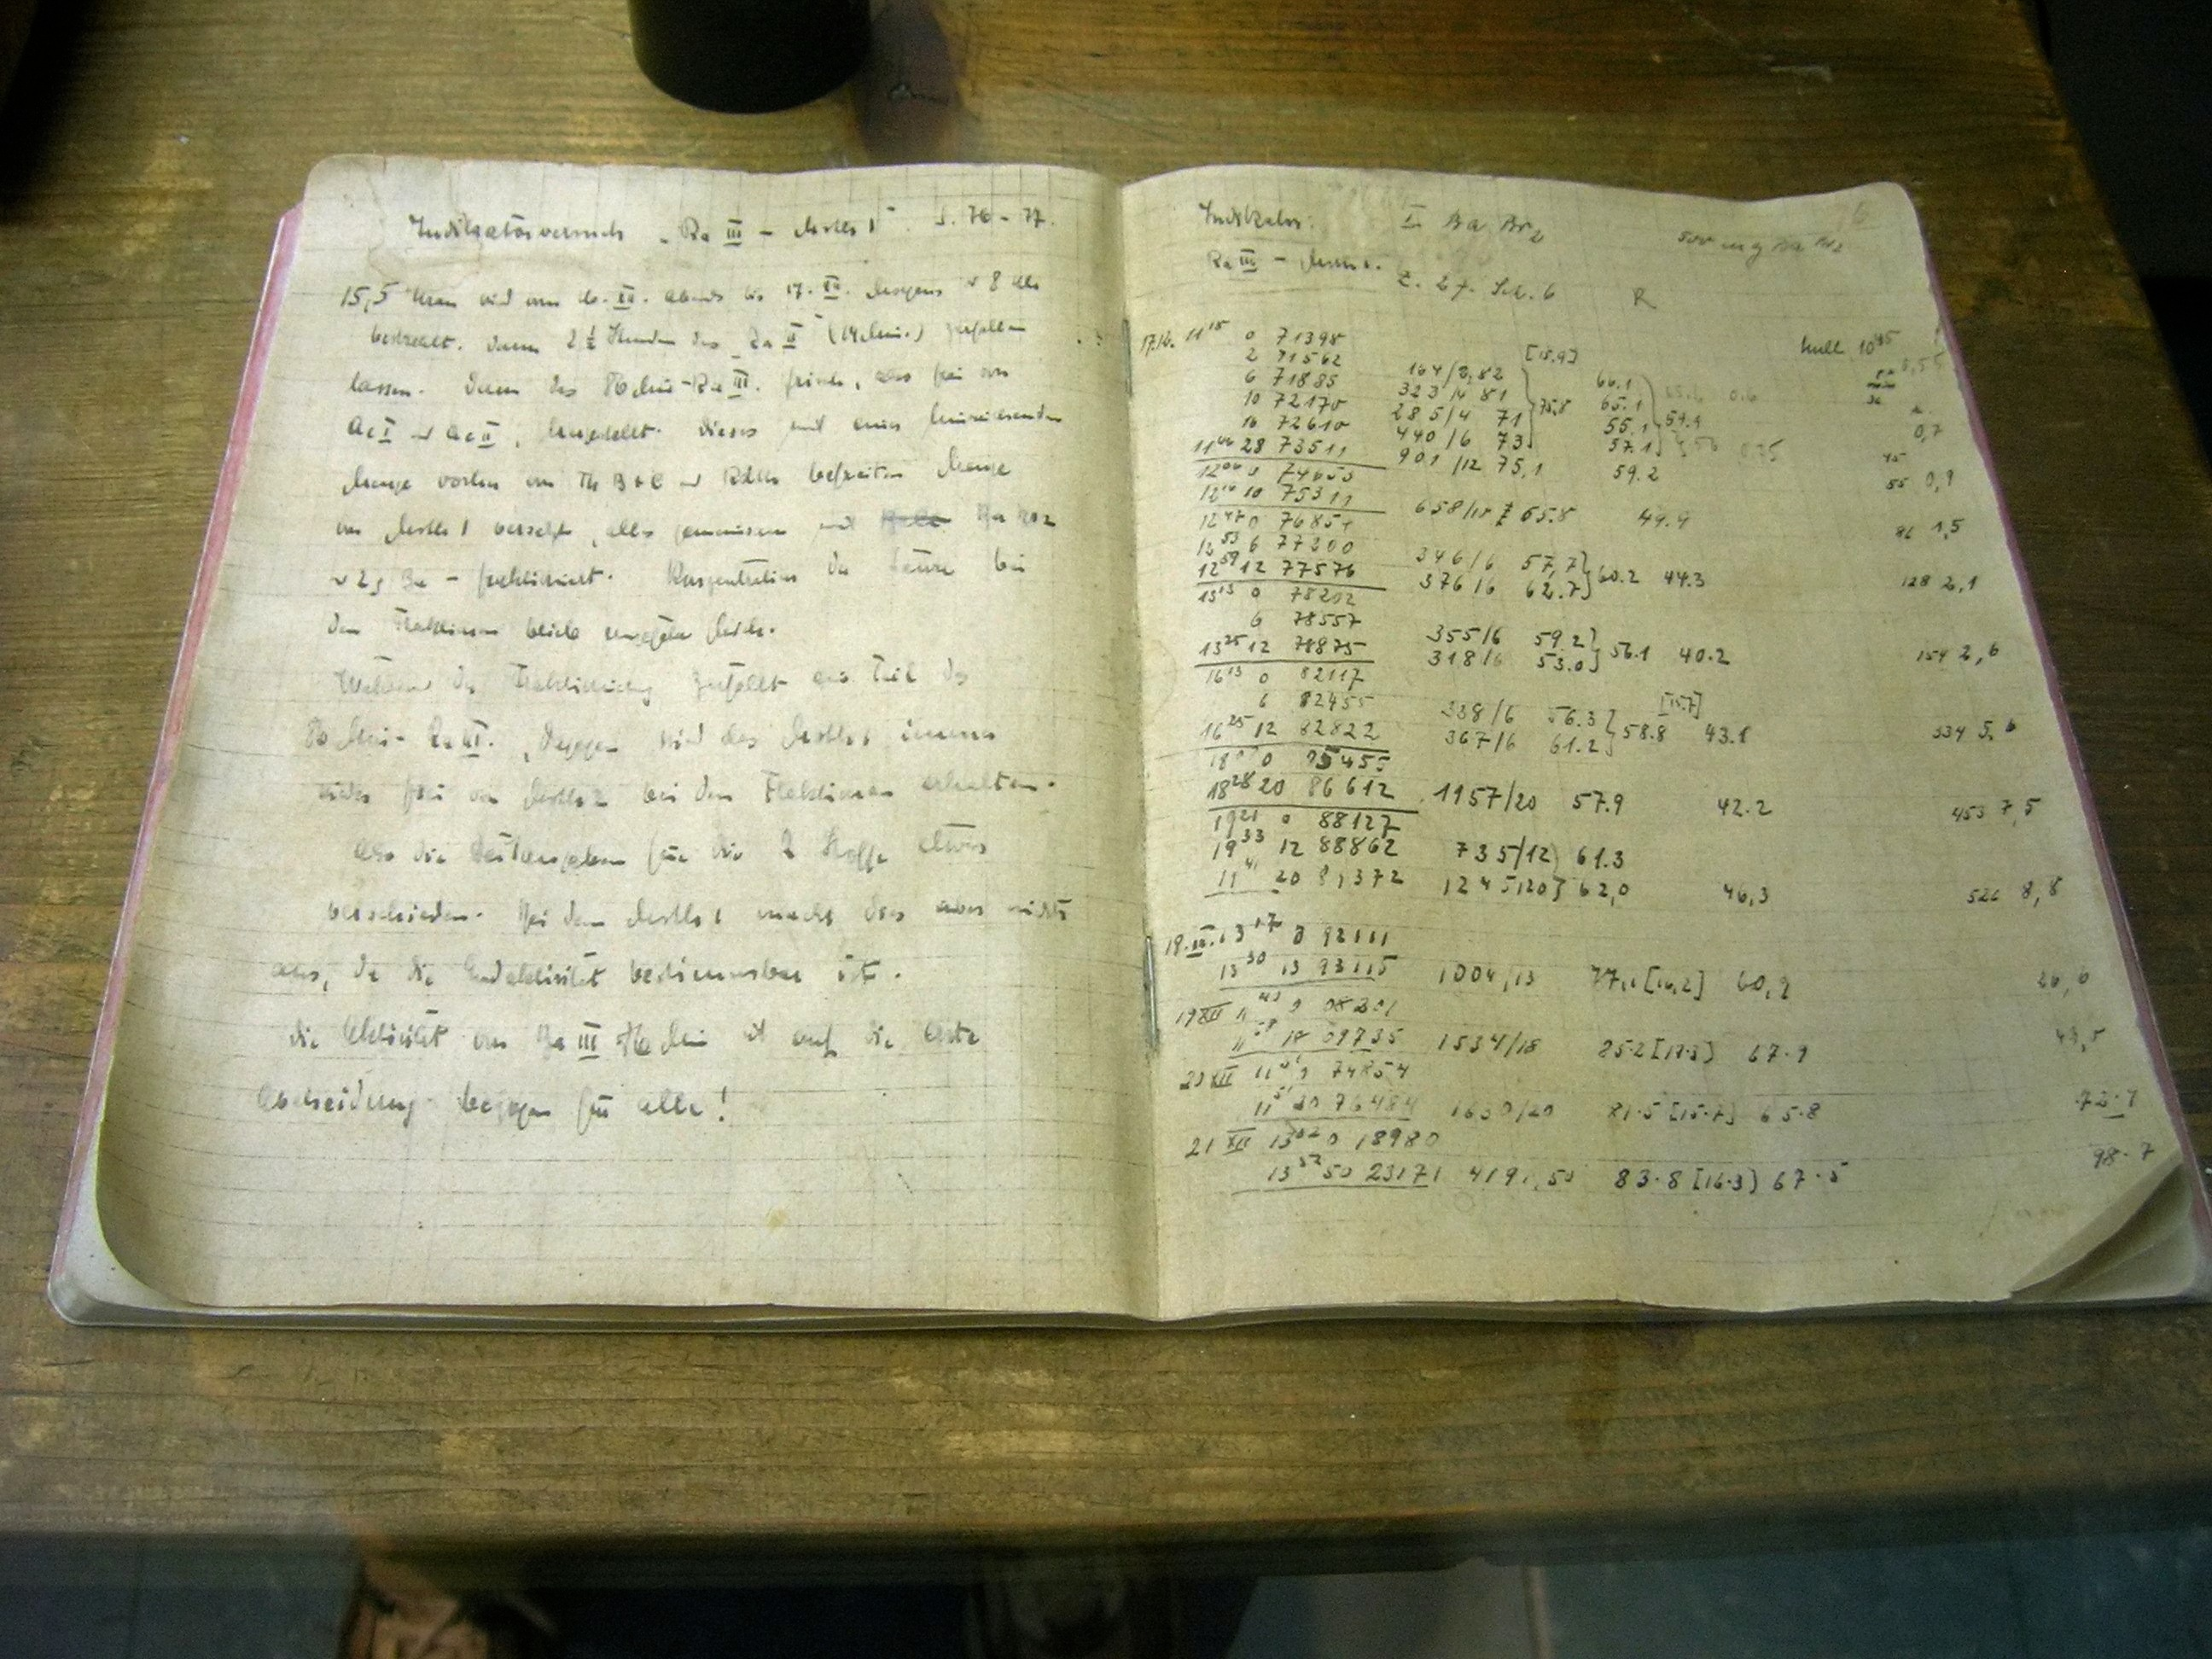
\includegraphics[width = 0.95\textwidth]{../labnotes/labnotes01}
    \caption{Laborheft Seite 1: Otto Hahn's notebook from exhibit of the Experimental Apparatus with which the team of Otto Hahn, Lise Meitner and Fritz Strassmann discovered Nuclear Fission in 1938.(\url{https://de.wikipedia.org/wiki/Laborjournal})}
    \label{fig:labnotes1}
\end{figure}




	\newpage
	\section{Erklärung zur Arbeitsteilung}
Alle Autor*en haben zu allen Inhalten des Protokolls zu gleichen Teilen beigetragen.


	%%%%%%%%%%%%%%%%%%%%%

	\clearpage
	% Abbildungsverzeichnis
	\addcontentsline{toc}{section}{Abbildungsverzeichnis}
	\listoffigures
	% Tabellenverzeichnis
	\addcontentsline{toc}{section}{Tabellenverzeichnis}
	\listoftables

	% Literaturverzeichnis
	\addcontentsline{toc}{section}{Literaturverzeichnis}
	\bibliographystyle{unsrt}
	\bibliography{bibliography.bib} %in der Datei bibliography. bib wird die Literatur eingetragen. Erst wenn sie mit \cite{bibid} im Text zitiert wird, taucht sie auch im Literaturverzeichnis auf.
\end{document}